\documentclass[10pt, a4paper]{beamer}

\usetheme{Berkeley}
\usecolortheme{sidebartab}
\usepackage{array}

\begin{document}
	\setbeamertemplate{sidebar left}{}
	\title{Progress Presentation-I}
	\subtitle{e-Yantra Summer Internship-2015 \\ IoT Connected valves for irrigation of greenhouse}
	\author{ Jayant Solanki \\ Kevin Dsouza\\ \vspace{0.5cm}
	\underline{Mentors} \\ Ajit Harpude \\Vishwanathan Iyer\\}
	\institute{KReSIT, IIT Bombay}
	\date{\today}
	%\addtobeamertemplate{sidebar left}{}{\includegraphics[scale = 0.3]{logowithtext.png}}
	\frame{\titlepage}

\setbeamertemplate{sidebar left}[sidebar theme]
\section{Overview of Project}
\begin{frame}{Overview of Project}
	\begin{itemize}
		\item Project name : IoT Connected valves for irrigation of greenhouse
		\item Objective : Development of a IOT based low-cost, low-power, standalone module for the automation of Irrigation in a greenhouse.
	        \item Deliverables : 
		\begin{itemize}
		\item Demonstration of control of valves remotely
                \item Detailed report on power consumption of the system
                \item Detailed report of the design process with documented code
                \end{itemize}
	\end{itemize}
\end{frame}

\section{Overview of Task}
\begin{frame}{Overview of Task}
        \centering 
	\begin{tabular}{|m{0.6cm}|m{6cm}|m{2cm}|}
	\hline
        sl.no& \centering Task & date of completion \\
        \hline
        1 & Finding appropriate WIFI module and communication protocol & June 2nd \\ \hline
        2 & Testing Solenoid,H-bridge and ESP8266 control circuit & June 3rd \\ \hline
        3 & Setting up and running openHAB server & June 6th \\ \hline
        4 & Controlling valves through MQTT broker & June 12th \\ \hline
        5 & Designing openHAB UI for controlling valves & June 13th \\ \hline
        6 & Look into sleep modes and last will testament Of ESP8266 &  \\ \hline
        7 & Adding features to the openHAB UI &  \\ \hline
        8 & New device discovery and data persistence & \\ \hline
        9 & To display the battery status of the connected device & \\ \hline 
        10 & Making a compact and portable design & \\ \hline
        \end{tabular}
\end{frame}

\section{Accomplished Tasks}
\begin{frame}[allowframebreaks,allowdisplaybreaks]{Accomplished Tasks}
        
	\begin{itemize}
		\item Survey on Latching solenoid valves and WIFI modules
		\begin{figure}
		 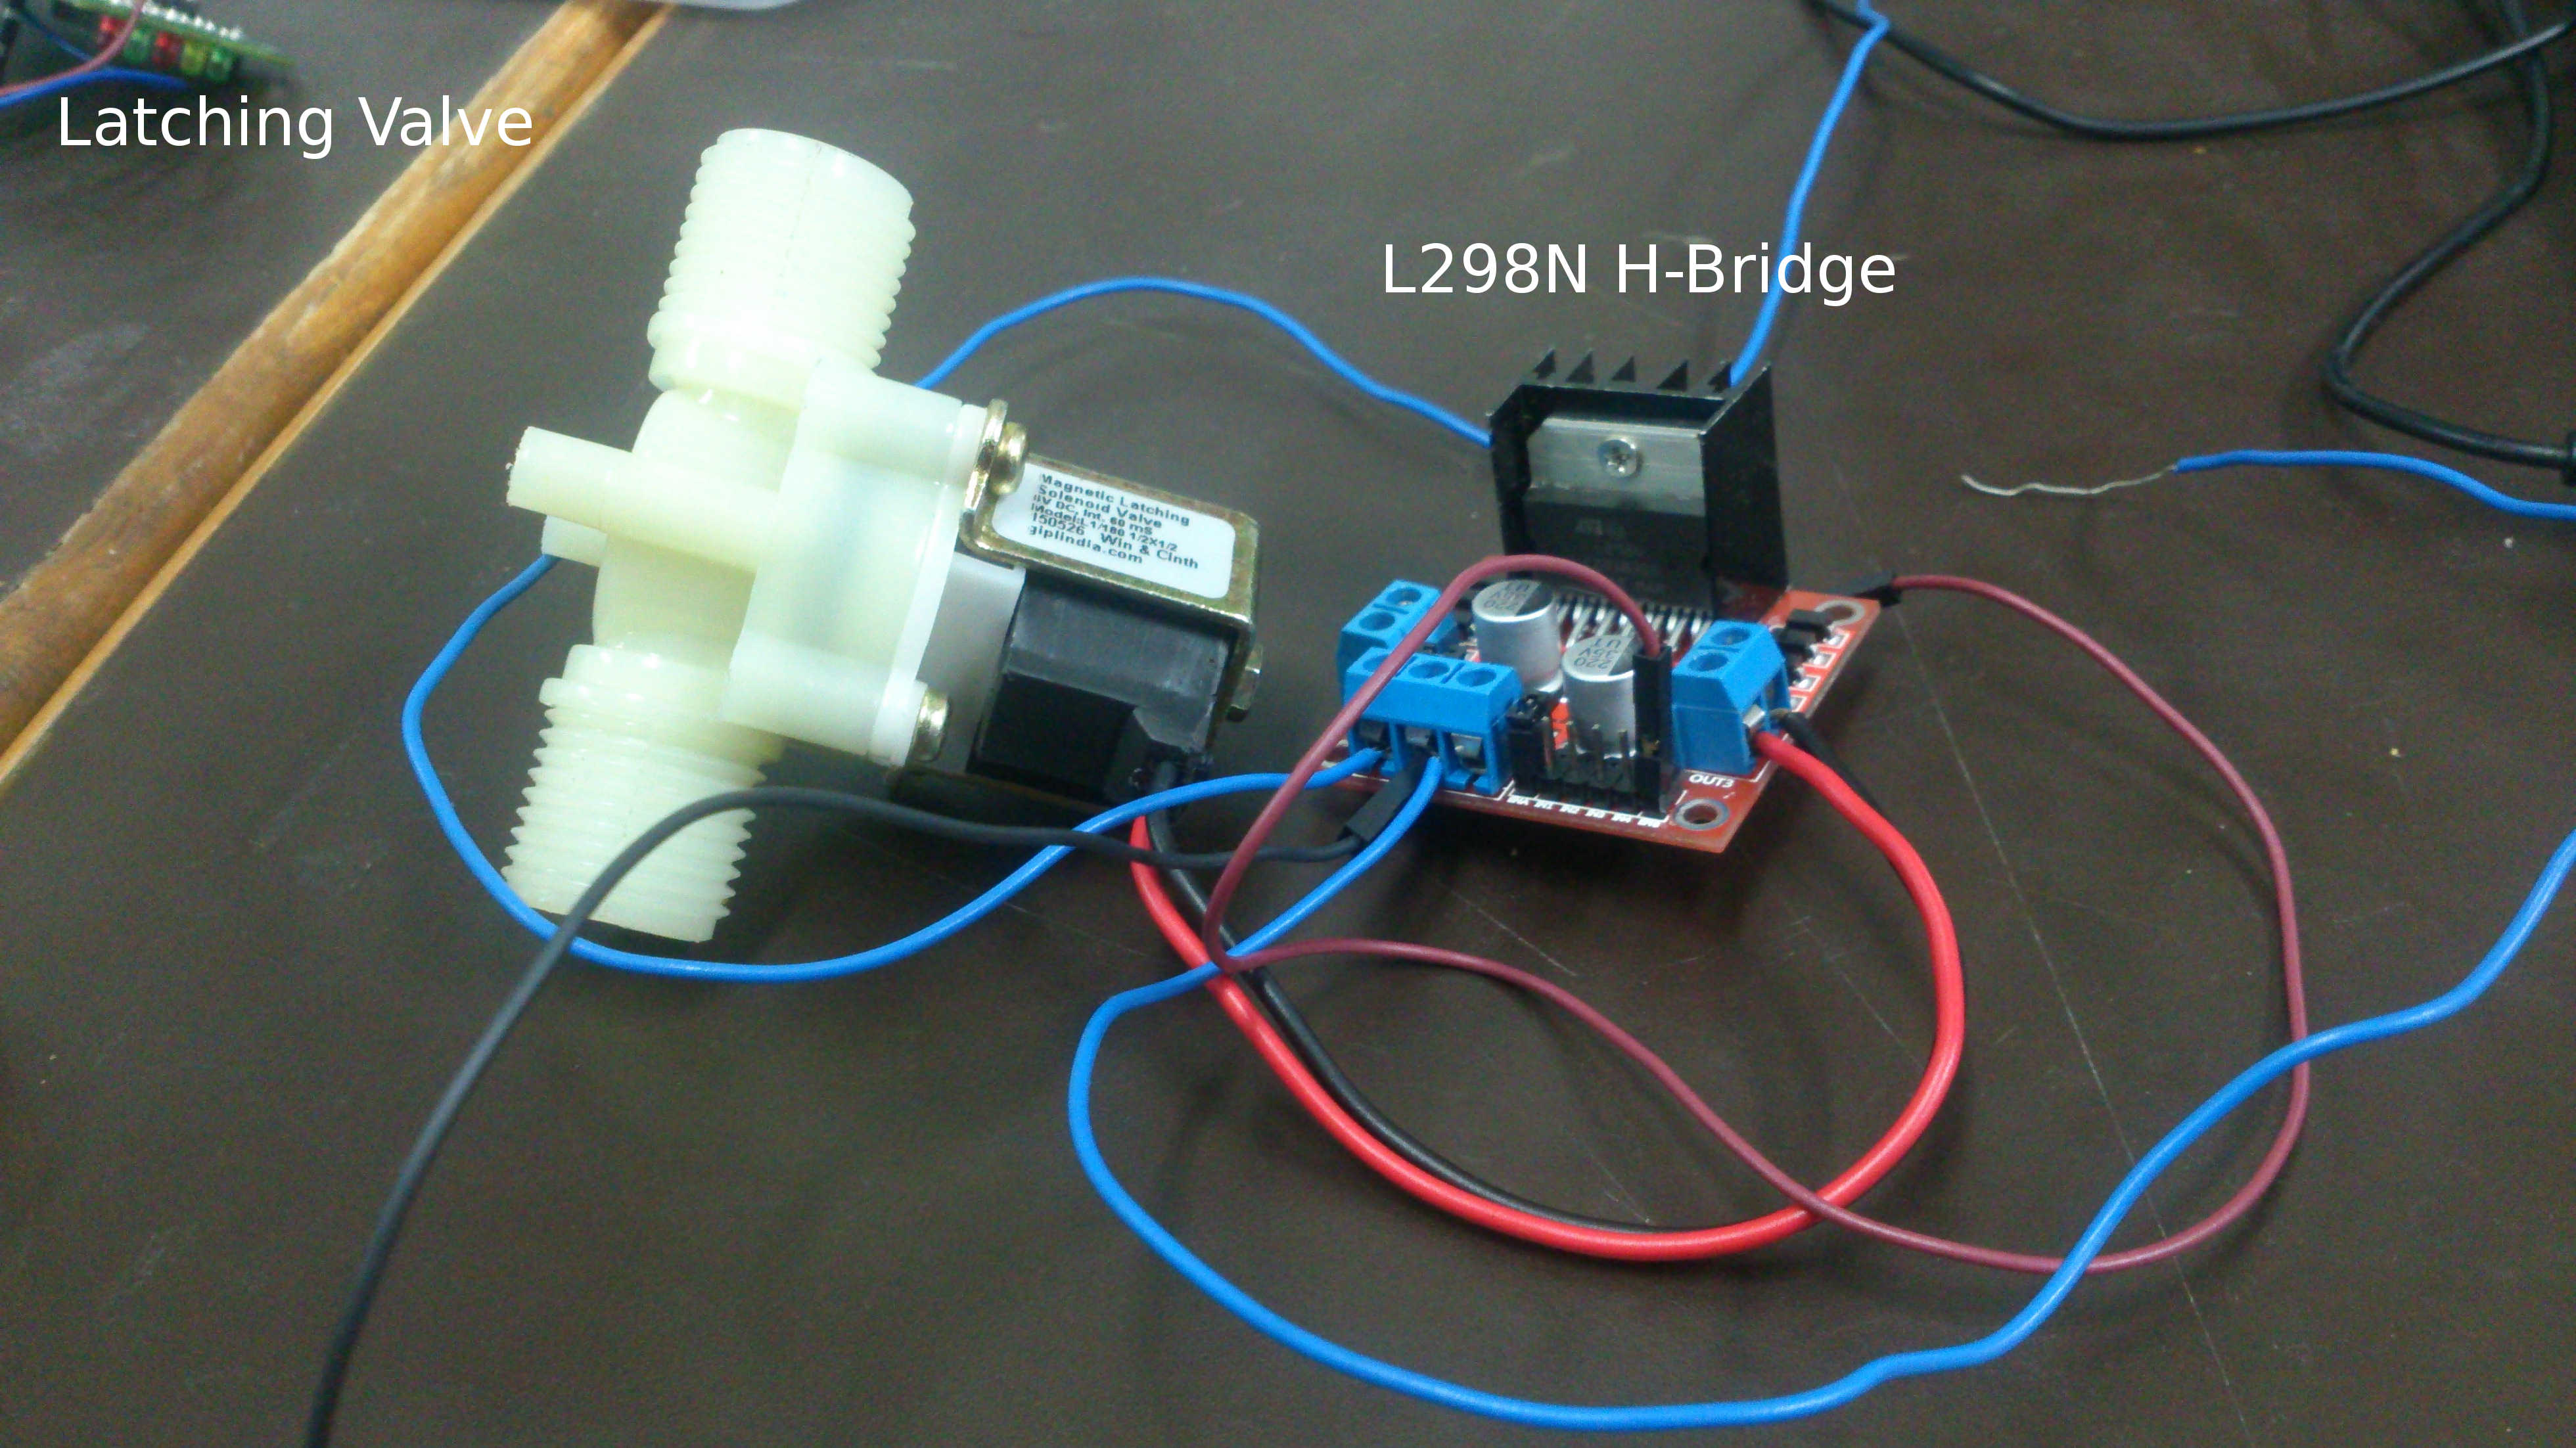
\includegraphics[width=3.5cm]{valve.jpg}
		\end{figure}
		\item Design and testing of circuit for controlling the valve
		\begin{figure}
		 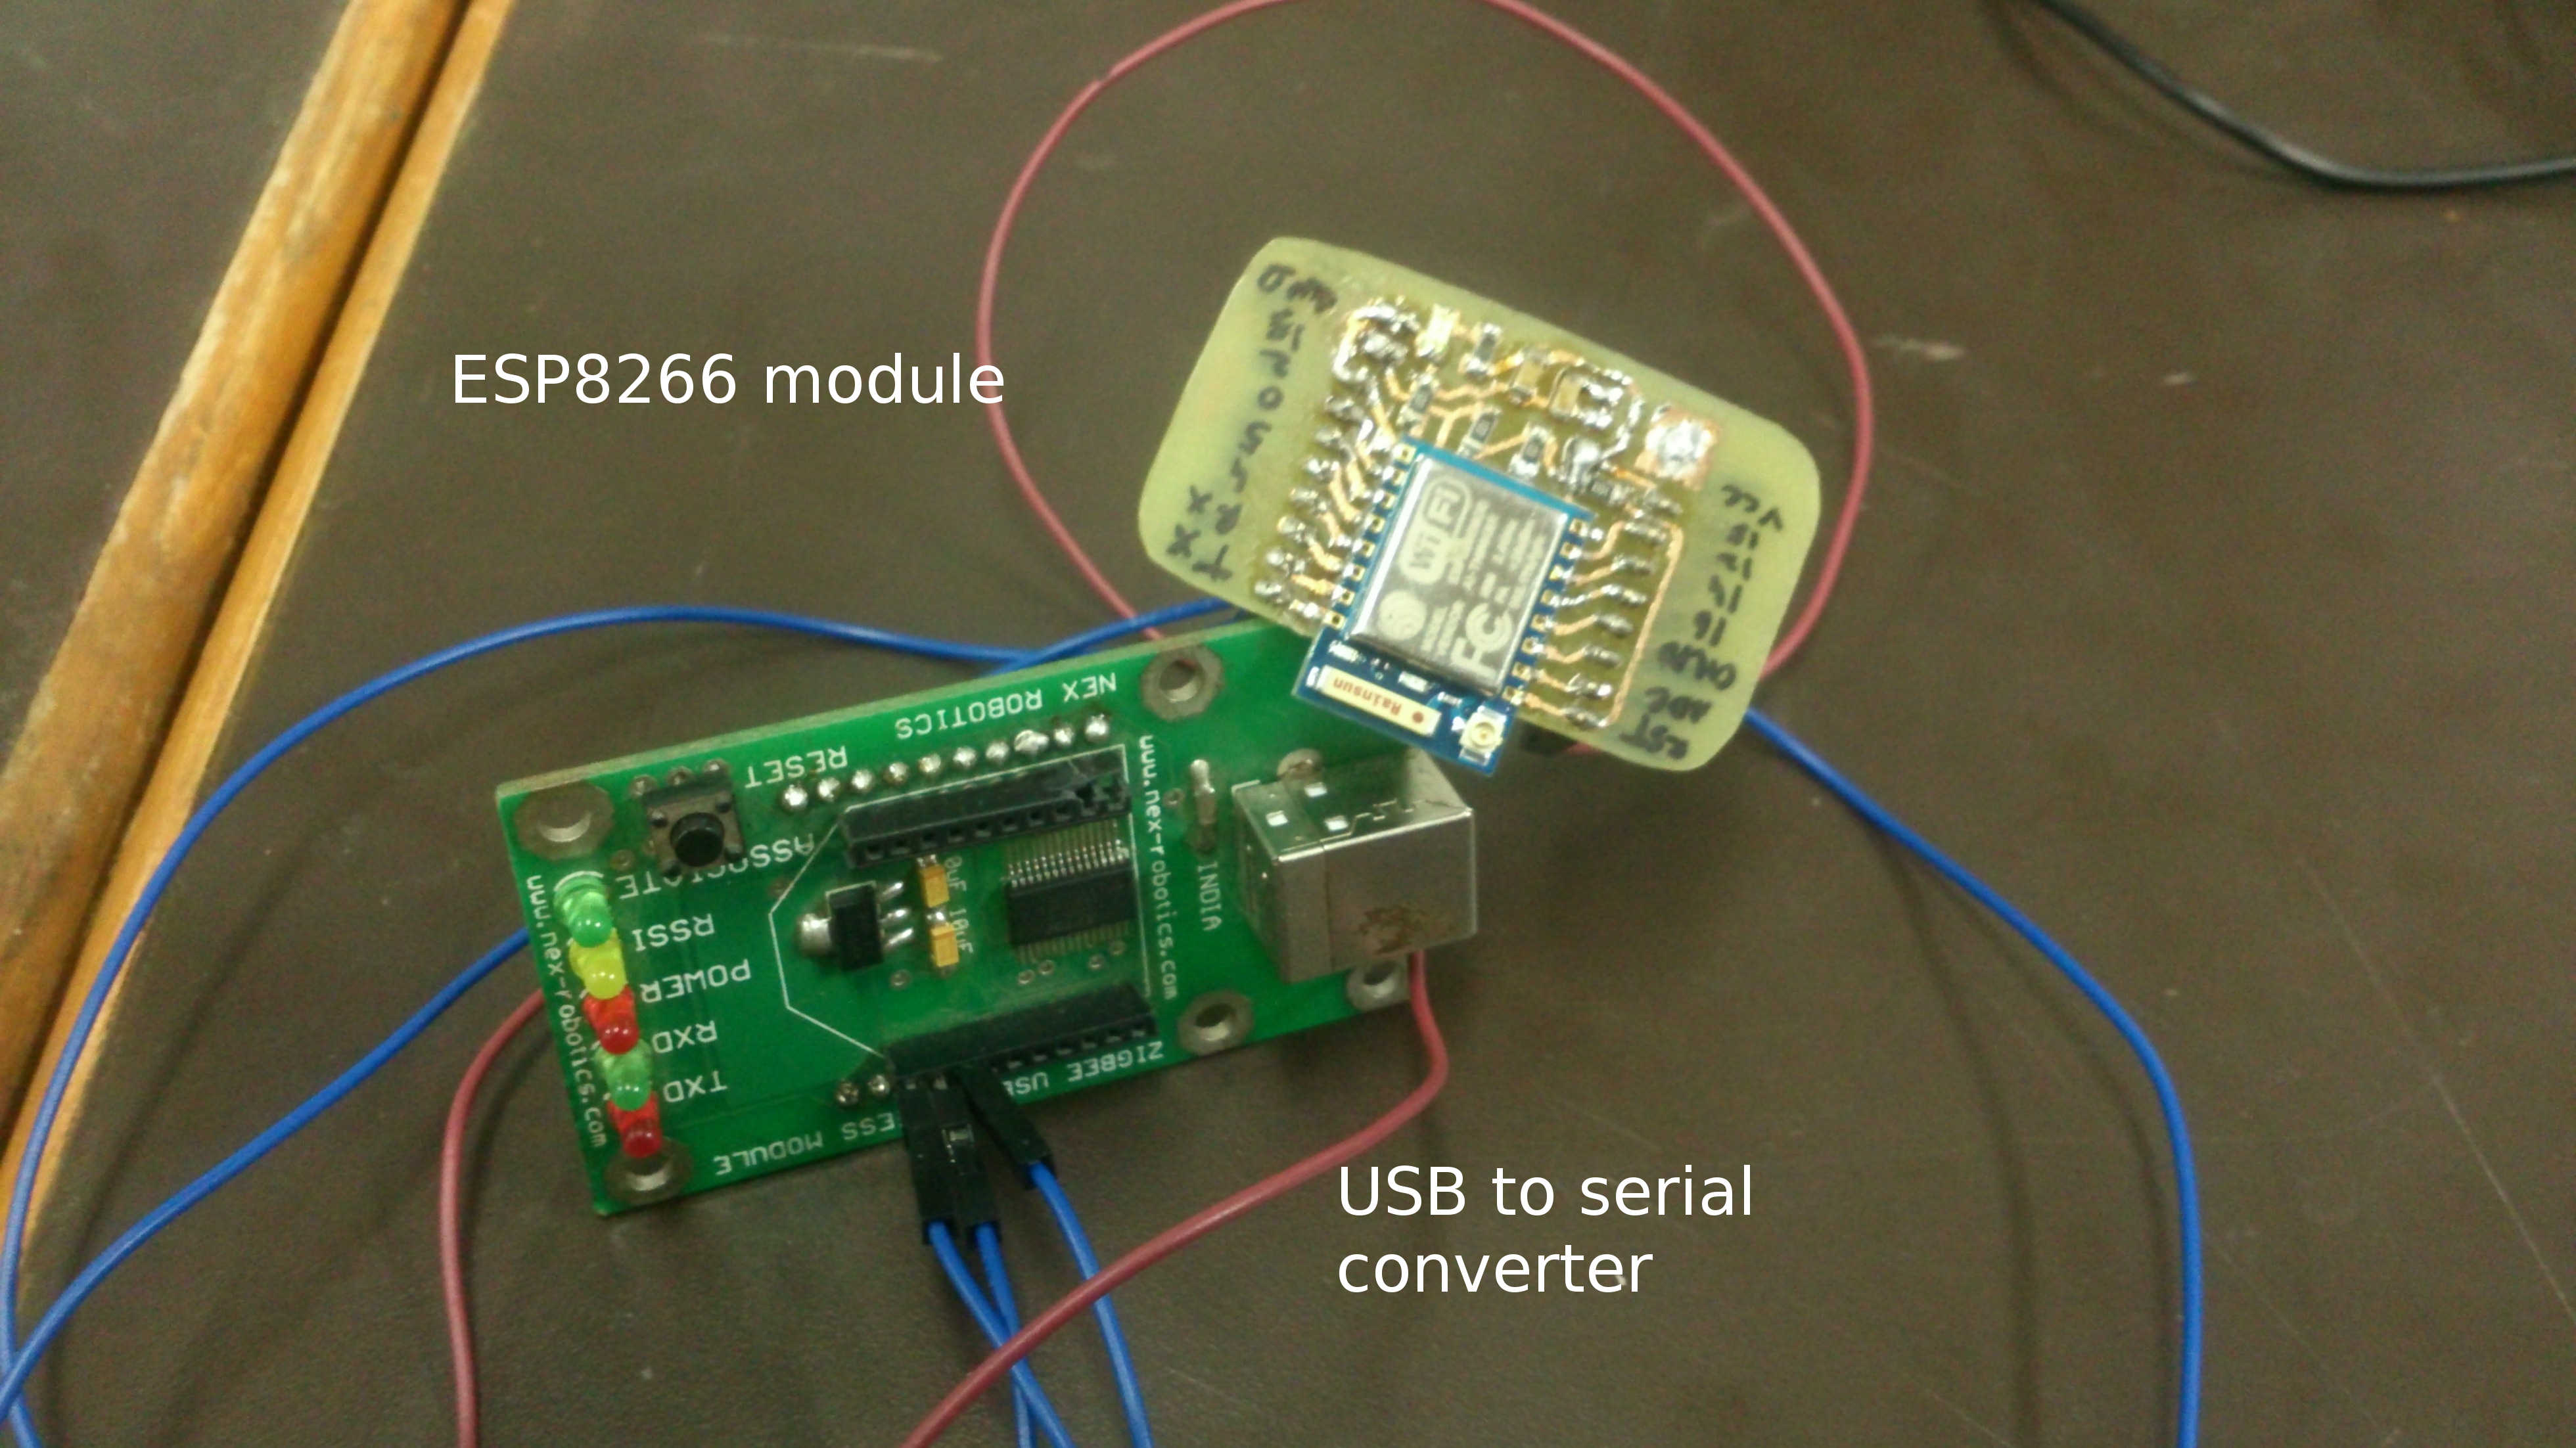
\includegraphics[width=3.5cm]{ESP8266.jpg}
		\end{figure}
		\item Survey on M2M communication protocol
		\item Remotely controlling the valves through ESP8266 
		\item Setting up openHAB and MQTT broker
		\item User interface to control the valves
		\begin{figure}
		 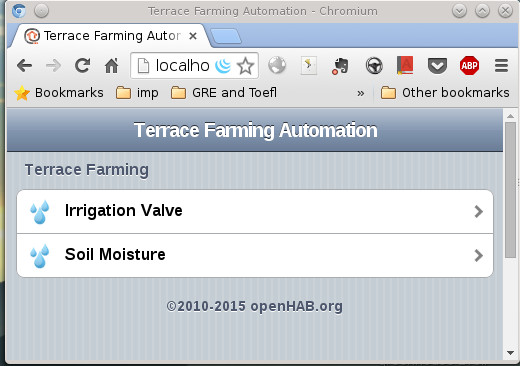
\includegraphics[width=3.5cm]{openhab.jpg} \hspace{1cm}
		 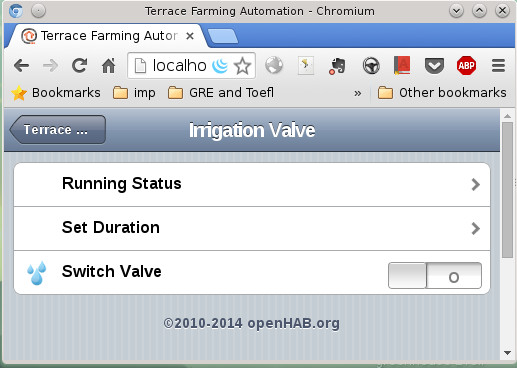
\includegraphics[width=3.5cm]{openhab2.jpg} \\ 
		  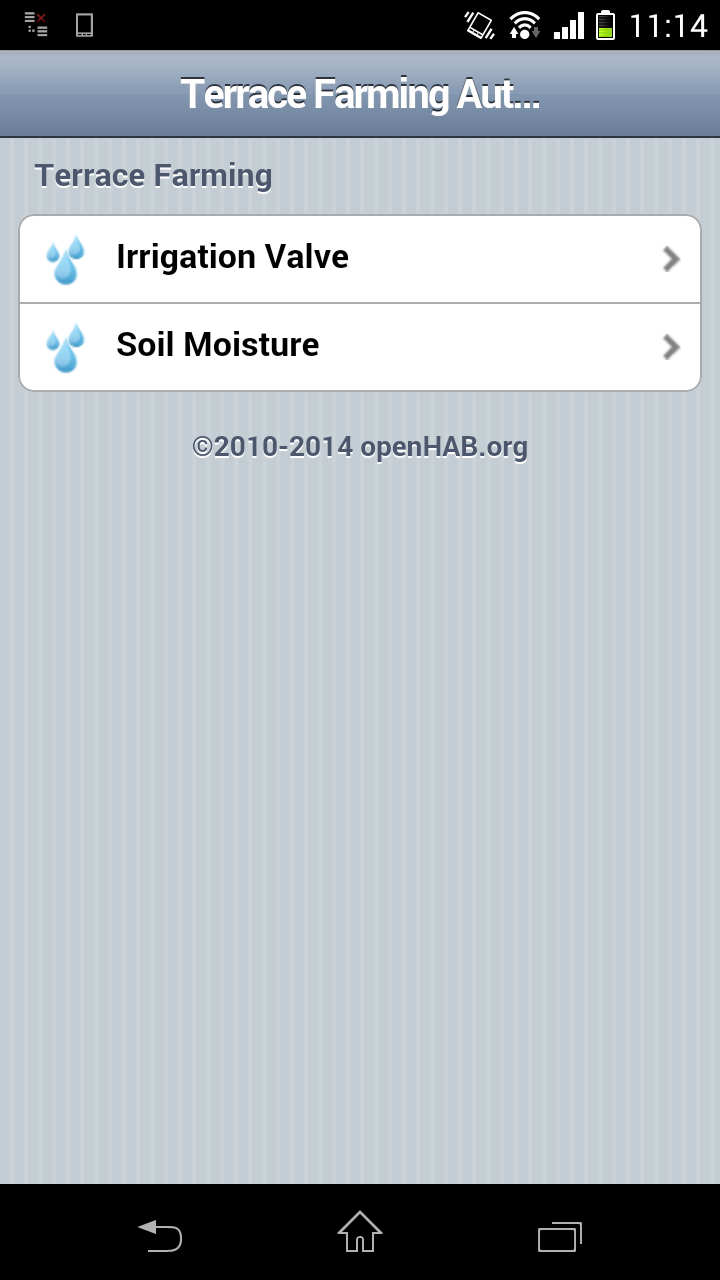
\includegraphics[width=3.5cm]{app1.jpg} \hspace{1cm}
		 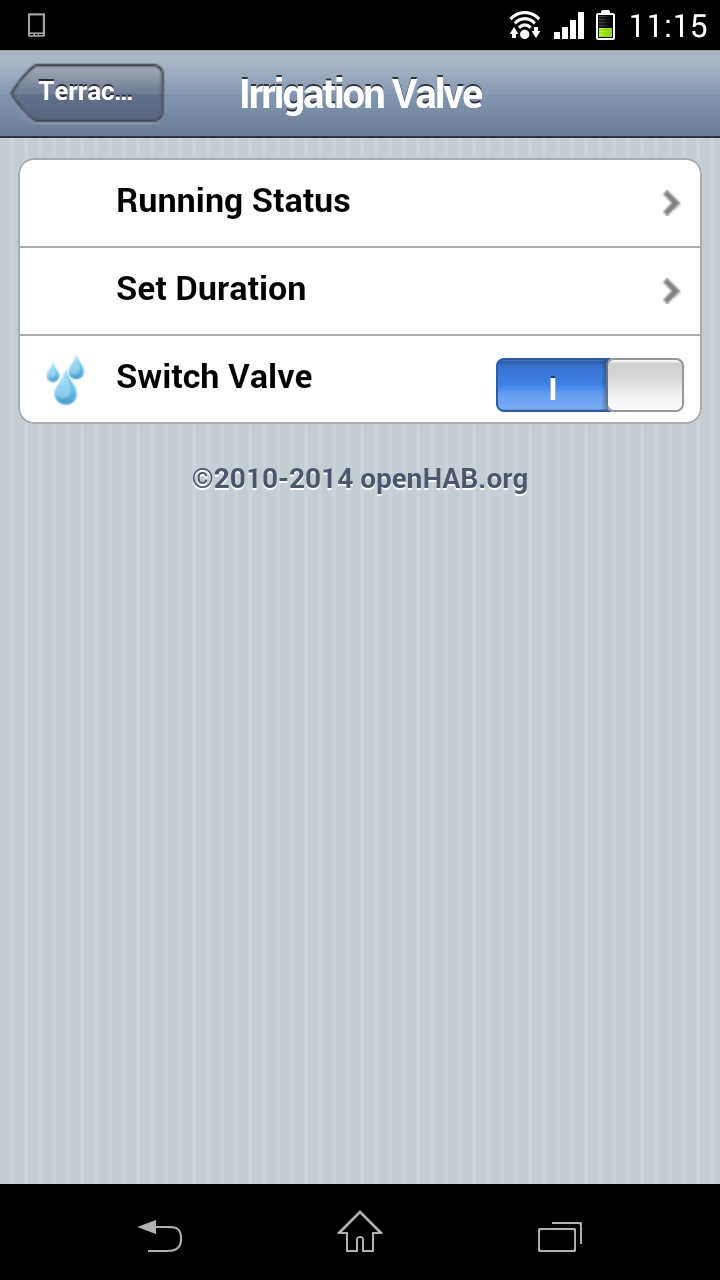
\includegraphics[width=3.5cm]{app2.jpg}\\
		 {\bf openHAB UI for android/IOS}
		\end{figure}
	\end{itemize}	
 
\end{frame}

\section{Pending Tasks}
\begin{frame}{Pending Tasks}
        \begin{itemize}
		\item Optimum power consumption design for the setup   
		\item Expanding UI features to timimg based operation and new device discovery
		\item Looking into 'last will and testament' function of the ESP8266
		\item Displaying battery status
		\item Making a compact,portable,plug\&play design for the setup 		
	\end{itemize}	
\end{frame}

\section{Challenges Faced}
\begin{frame}{Challenges Faced}
	\begin{itemize}
		\item Getting used to a fairly recent module ESP8266
		\item Deciding between nodeMCU and Arduino IDE
		\item Memory management in the ESP8266
		\item Power management in IOT applications
		\item Understanding openHAB,data persistence and bindings 
		\item Installation of MOSCA broker on linux system
	\end{itemize}
\end{frame}

\section{Current cost and future Plans}
\begin{frame}{Current cost and future Plans}
\begin{tabular}{|m{6cm}|m{3cm}|}
	\hline
	{\bf Items} & {\bf Est.cost in Rupees}\\ \hline
	ESP8266 & 400 \\ \hline
	Rechargible Alkaline battery & 150 \\ \hline
	H-bridge & 100 \\ \hline 
	Latching Solenoid valve & 430 \\ \hline
	Total cost & 1080 \\ \hline 
\end{tabular} 
\vspace{1cm}\\
\centering{\bf Future plans} \\
	\begin{itemize}
		\item Integrating Solar power with the module
		\item Including a water flow meter sensor
		\item Including soil moisture sensors and control valves accordingly
	\end{itemize}
\end{frame}


\section{Thank You}
\begin{frame}{Thank You}
	\hspace{4cm} Thank you !!!
\end{frame}
\end{document}
